\subsubsection{Giới thiệu bộ dữ liệu}
    \paragraph{Nguồn dữ liệu}
    \leavevmode

    Đây là bộ dữ liệu giá cổ phiếu Hòa Phát Group (HPG) nhóm tự thu thập từ api cafef.vn.

    \paragraph{Mô tả dữ liệu}
    \leavevmode
    Mỗi dòng dữ liệu chứa thông tin giá cổ phiếu HPG. Khoảng dữ liệu từ này 15/11/2007 đến ngày 20/06/2025.

    Ví dụ một phần dữ liệu:

    \begin{table}[htbp]
    \centering
    \caption{Một phần bảng dữ liệu giá cổ phiếu HPG}
    \label{tab:stat-stock-exp}
        \begin{tabular}{|l|r|r|r|r|r|r|}
        \hline
        Ngay & GiaDieuChinh & GiaDongCua & GiaMoCua & GiaCaoNhat & GiaThapNhat & ... \\
        \hline
        15/11/2007 & 2.40 & 127.00 & 130.00 & 130.00 & 109.00 & ... \\
        \hline
        16/11/2007 & 2.29 & 121.00 & 121.00 & 121.00 & 121.00 & ... \\
        \hline
        19/11/2007 & 2.17 & 115.00 & 115.00 & 115.00 & 115.00 & ... \\
        \hline
        20/11/2007 & 2.08 & 110.00 & 110.00 & 110.00 & 110.00 & ... \\
        \hline
        ... & ... & ... & ... & ... & ... & ... \\
        \hline
        \end{tabular}

    \end{table}

     Bộ dữ liệu có 4384 dòng, bao gồm 14  cột như sau:

    \begin{itemize}
        \item Kiểu dữ liệu: \textbf{Qualitative} 
        \begin{enumerate}
            \item \textbf{Stock}: Mã cổ phiếu, HPG
        \end{enumerate}
    
        \item Kiểu dữ liệu: \textbf{Quantitative} 
        \begin{itemize}
            \item \textbf{Continuous}:
             \begin{enumerate}[resume]
                \item \textbf{Ngay}: Ngày

                \item \textbf{GiaDieuChinh}: Giá điều chỉnh
 
                \item \textbf{GiaDongCua}: Giá đóng cửa

                \item \textbf{GiaMoCua}: Giá mở cửa

                \item \textbf{GiaCaoNhat}: Giá cao nhất

                \item \textbf{GiaCaoNhat}: Giá cao nhất
                \item \textbf{GiaThapNhat}: Giá thấp nhất
    
                \item \textbf{ThayDoi}: Giá thay đổi và tỉ lệ thay đổi giữa giá mở - đóng
                
                \item \textbf{GiaThayDoi}: Giá thay đổi (Thay đổi giữa giá mở - đóng)
                \item \textbf{ThayDoiPhanTram}: Tỉ lệ thay đổi giữa giá mở - đóng
                \item \textbf{KhoiLuongKhopLenh}: Khối lượng cổ phiếu giao dịch
                \item \textbf{GiaTriKhopLenh}: Giá tổng số cổ phiếu giao dịch
                \item \textbf{KLThoaThuan}: Khối lượng thỏa thuận (khối lượng dự kiến trước giao dịch)
                \item \textbf{GtThoaThuan}: Giá trị thỏa thuận (giá trị dự kiến trước giao dịch)
            \end{enumerate}

        \end{itemize}

    \end{itemize}

\subsubsection{Phân tích dữ liệu}
    \paragraph{Thống kê dữ liệu}
        \leavevmode

    Bảng \ref{tab:stat-stock} thể hiện các thông số thống kê trên một số đặc trưng của bộ dữ liệu.

    \begin{table}[htbp]
    \centering
    \caption{ Thống kê dữ liệu một số đặc trưng dữ liệu giá chứng khoán HPG}
    \label{tab:stat-stock}
    \begin{tabular}{|l|l|l|l|l|}
    \hline
      & GiaDieuChinh & GiaDongCua & ThayDoiPhanTram & KhoiLuongKhopLenh \\
    \hline
    Mean & 10.1627 & 37.4874 & 0.0599 & $8.1*10^6$ \\
    \hline
    Min & 0.68 & 12.1 & -22.86 & 0 \\
    \hline
    Q1 & 1.79 & 26.45 & -1.11 & 472,235 \\
    \hline
    Median & 5.73 & 32.7 & 0 & 2,542,830 \\
    \hline
    Q3 & 17.035 & 45.95 & 1.2425 & 12,830,875 \\
    \hline
    Max & 39.9 & 127 & 7 & 99,658,800 \\
    \hline
    Mode & 1.17 & 23 & 0 & 0 \\
    \hline
    Var & 104.3475 & 238.1792 & 5.284 & $137*10^{12}$ \\
    \hline
    SD & 10.2151 & 15.4331 & 2.2987 & $11.7*10^6$ \\
    \hline
    CV & 1.0051 & 0.4117 & 38.3627 & 1.4354 \\
    \hline
    IQR & 15.245 & 19.5 & 2.3525 & 12,358,640 \\
    \hline
    \end{tabular}
    \end{table}

    Từ đây, ta có thể rút ra một số nhận xét:

    \begin{itemize}
    \item GiaDieuChinh:  Giá điều chỉnh có trung bình 10.16 nhưng trung vị chỉ 5.73 và mode là 1.17, cho thấy phần lớn phiên giao dịch có mức giá thấp, trong khi một số ít phiên có giá rất cao kéo trung bình lên. Biến thiên lớn được thể hiện qua độ lệch chuẩn 10.21 và hệ số biến thiên > 1 (CV = 1.0051), phản ánh sự phân tán dữ liệu mạnh và phân phối lệch phải rõ rệt.
    
    \item GiaDongCua: Mức giá đóng cửa có trung bình 37.49, trung vị 32.7 và mode là 23, phản ánh sự chênh lệch giá giữa các giai đoạn. Dữ liệu dao động trong khoảng 12.1 đến 127, với độ lệch chuẩn khá lớn (15.43). Tuy nhiên, hệ số biến thiên (CV = 0.41) ở mức vừa phải, cho thấy giá biến động nhưng không quá cực đoan nếu so với giá trị trung bình.
    
    \item ThayDoiPhanTram: Mức thay đổi phần trăm theo ngày có trung bình gần 0 ($\approx$ 0.06), cho thấy giá thường đi ngang hoặc biến động nhỏ. Tuy nhiên, giá trị min = –22.86\% và max = 7\% cho thấy vẫn có các phiên biến động rất mạnh. Mode = 0 càng củng cố việc thị trường thường ít thay đổi trong ngắn hạn.
    
    \item KhoiLuongKhopLenh:
    Trung bình khối lượng khớp lệnh là 8.1 triệu cổ phiếu, nhưng trung vị chỉ khoảng 2.54 triệu và mode bằng 0 cho thấy có rất nhiều phiên giao dịch với thanh khoản thấp, bị kéo lên bởi một số phiên có khối lượng cực lớn (max $\approx$ 100 triệu). Độ lệch chuẩn cao ($\approx 11.7$ triệu) và CV = 1.43 phản ánh tính chất cực kỳ không ổn định của biến này.
    
    \end{itemize}

    \paragraph{Trực quan hóa dữ liệu}
    \leavevmode

    \begin{figure}[htp]
        \centering
        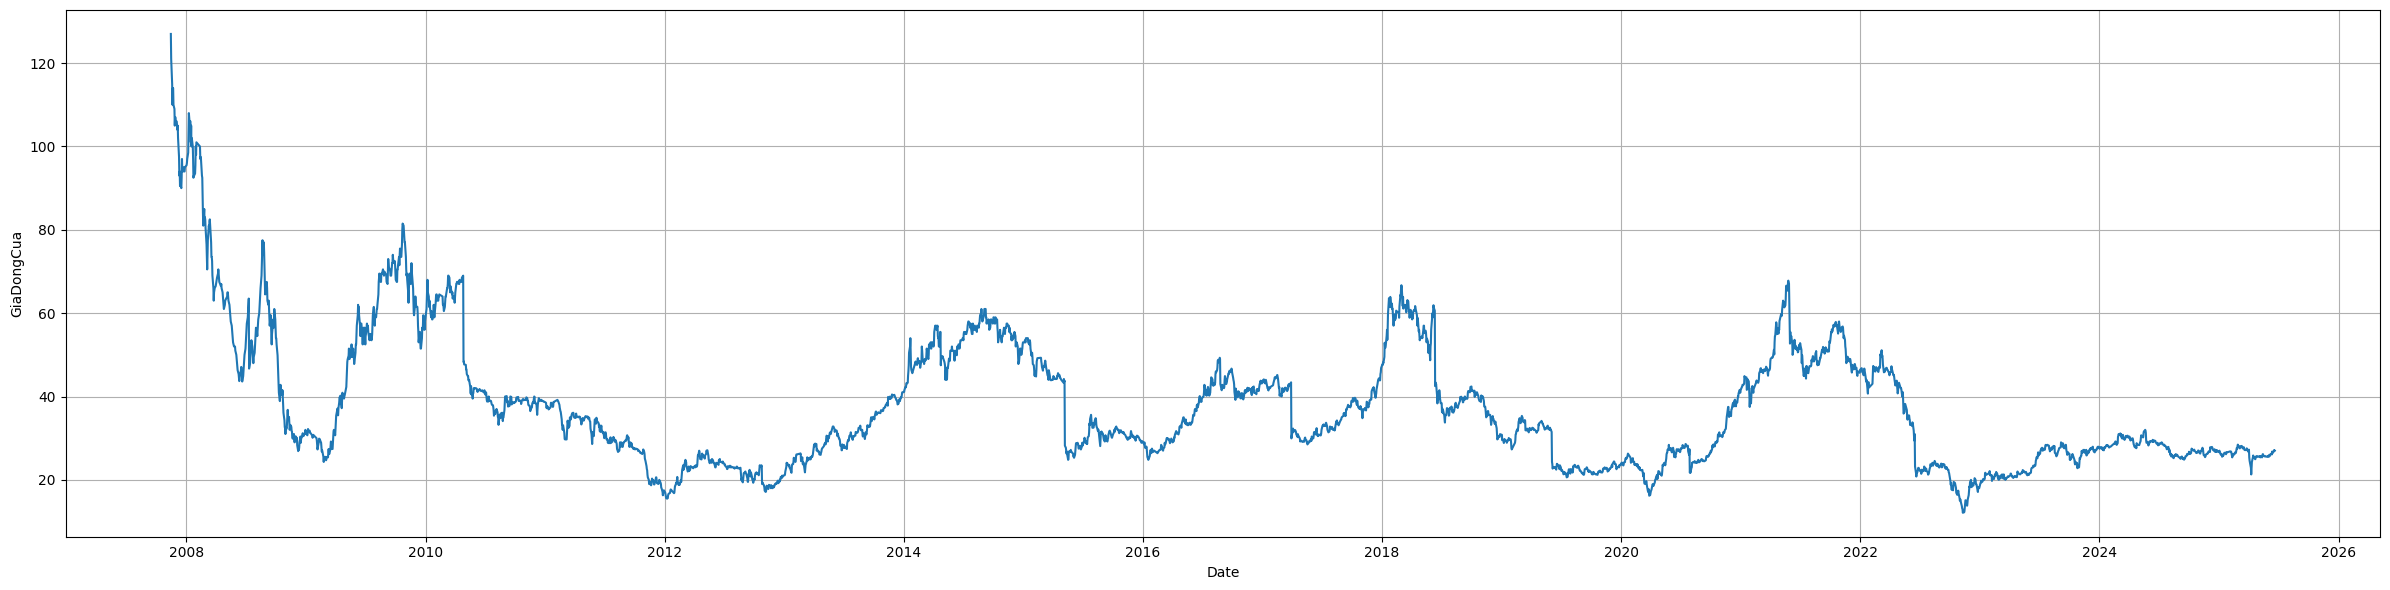
\includegraphics[width=0.90\textwidth]{images/TS_stock_close.png}
        \caption{Giá đóng cửa theo thời gian}
        \label{fig:TS_stock_close}
    \end{figure}
    \FloatBarrier

    Biểu đồ \ref{fig:TS_stock_close} thể hiện biến động giá đóng cửa của cổ phiếu trong giai đoạn dài từ 2007 đến 2025. Giá có xu hướng giảm mạnh ở giai đoạn đầu, sau đó dao động lên xuống theo chu kỳ nhưng không duy trì được xu hướng tăng dài hạn. Trong những năm gần đây, giá có dấu hiệu ổn định hơn và biến động nhẹ quanh một mức nhất định. Nhìn chung, biểu đồ cho thấy cổ phiếu trải qua nhiều biến động lớn, nhưng hiện tại đang trong trạng thái bình ổn.

    \begin{figure}[htp]
        \centering
        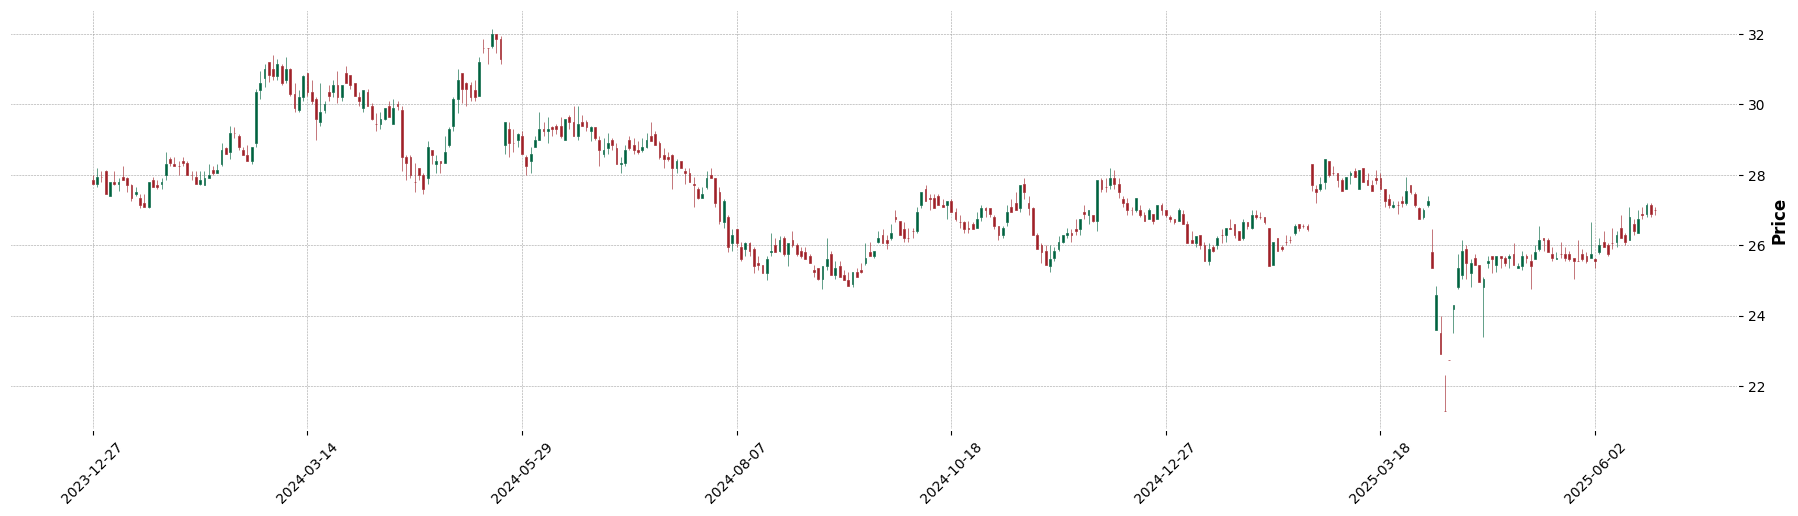
\includegraphics[width=0.90\textwidth]{images/TS_stock_close_candle_365.png}
        \caption{Giá hình nến theo thời gian - 365 ngày gần nhất}
        \label{fig:TS_stock_close_candle_365}
    \end{figure}
    \FloatBarrier

     Biểu đồ \ref{fig:TS_stock_close_candle_365} thể hiện biến động giá cổ phiếu HPG theo cây nến, trong một năm gần đây nhất. 

     \begin{figure}[htp]
        \centering
        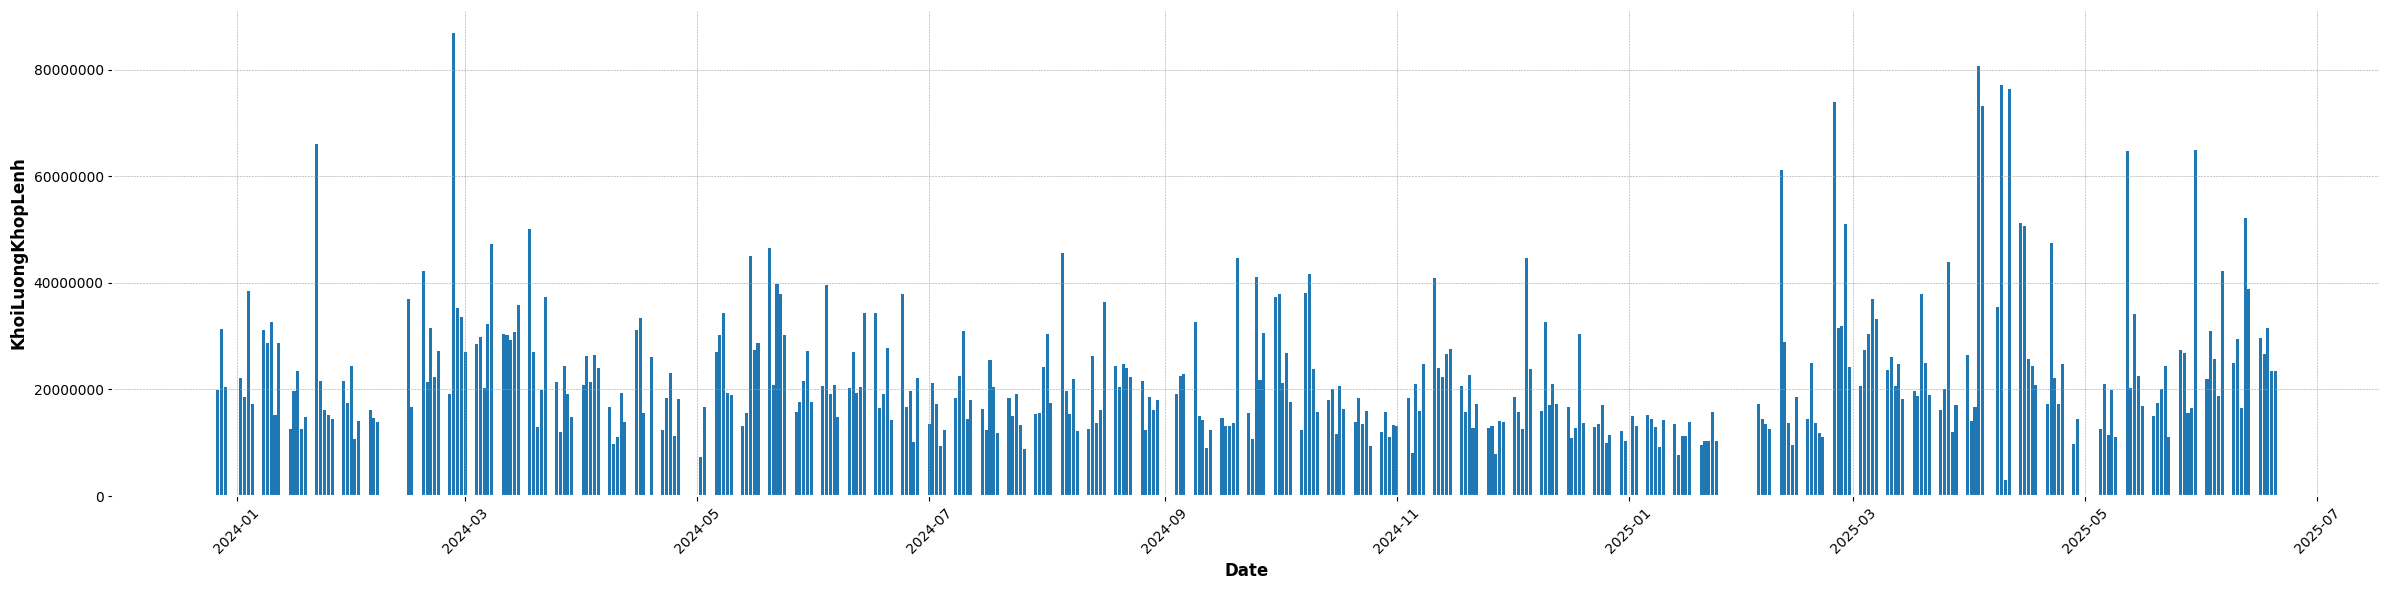
\includegraphics[width=0.90\textwidth]{images/TS_stock_volumn_365.png}
        \caption{Khối lượng khớp lệnh theo thời gian - 365 ngày gần nhất}
        \label{fig:TS_stock_volumn_365}
    \end{figure}
    \FloatBarrier

    Biểu đồ \ref{fig:TS_stock_volumn_365} thể hiện khối lượng khớp lệnh cổ phiếu HPG trong một năm gần đây nhất. Khối lượng giao dịch biến động mạnh, với nhiều đợt tăng vọt xuất hiện rải rác trong toàn bộ giai đoạn. Một số phiên có khối lượng cao, cho thấy những thời điểm giao dịch sôi động bất thường. Có những đoạn không có khối lượng giao dịch là ngày thị trường không giao dịch (ngày nghỉ).

    \begin{figure}[htp]
        \centering
        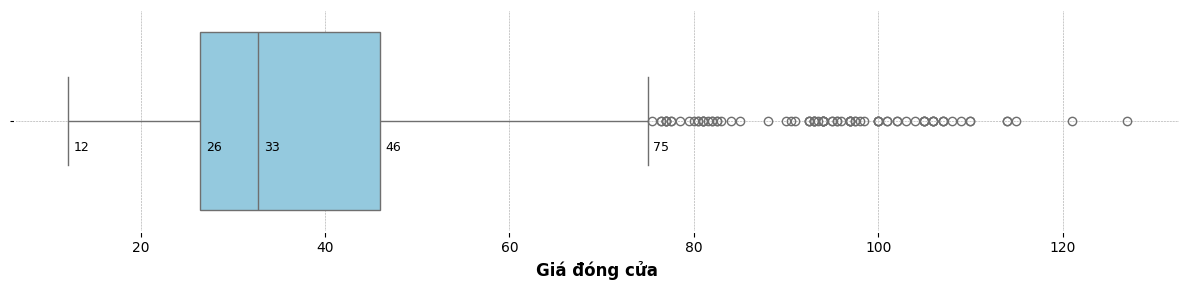
\includegraphics[width=0.90\textwidth]{images/TS_stock_close_box.png}
        \caption{Giá đóng cửa}
        \label{fig:TS_stock_close_box}
    \end{figure}
    \FloatBarrier

    Biểu đồ \ref{fig:TS_stock_close_box} thể hiện phân bố giá đóng cửa của cổ phiếu có trung vị khoảng 33, với phần lớn giá trị nằm trong khoảng từ 26 đến 46. Điều này cho thấy giai đoạn phổ biến nhất của giá cổ phiếu dao động quanh vùng trung bình thấp. Tuy nhiên, bên phải có rất nhiều điểm ngoại lệ, kéo dài đến hơn 120, cho thấy đã từng có nhiều phiên giao dịch với giá cao bất thường. Phân bố lệch phải rõ rệt, tức là phần lớn thời gian cổ phiếu giao dịch ở mức thấp đến trung bình, nhưng có không ít lần tăng vọt lên mức rất cao.

    \begin{figure}[htp]
        \centering
        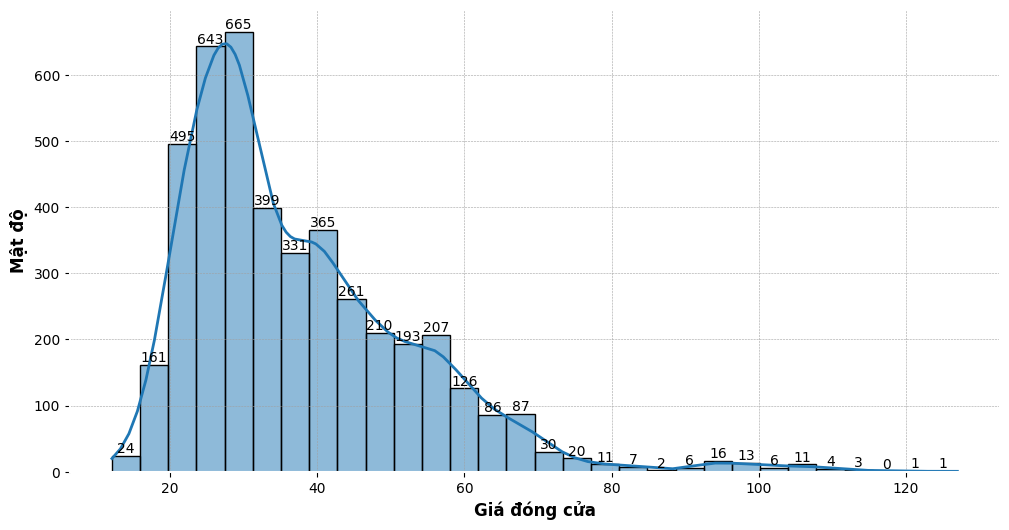
\includegraphics[width=0.90\textwidth]{images/TS_stock_close_hist.png}
        \caption{Phân phối giá đóng cửa}
        \label{fig:TS_stock_close_hist}
    \end{figure}
    \FloatBarrier

    Biểu đồ  \ref{fig:TS_stock_close_hist} cho thấy phần lớn cổ phiếu được giao dịch ở mức giá từ khoảng 25 đến 45, với đỉnh cao nhất rơi vào khoảng 28. Phía bên phải của phân phối kéo dài và thưa dần, cho thấy có một số phiên có giá đóng cửa rất cao, thậm chí vượt 100. Tuy nhiên, tần suất những mức giá này rất thấp. Điều này cho thấy phân phối có dạng lệch phải, phản ánh cổ phiếu chủ yếu được giao dịch ở mức giá thấp đến trung bình, và chỉ hiếm khi tăng mạnh lên vùng giá cao.

    \begin{figure}[htp]
        \centering
        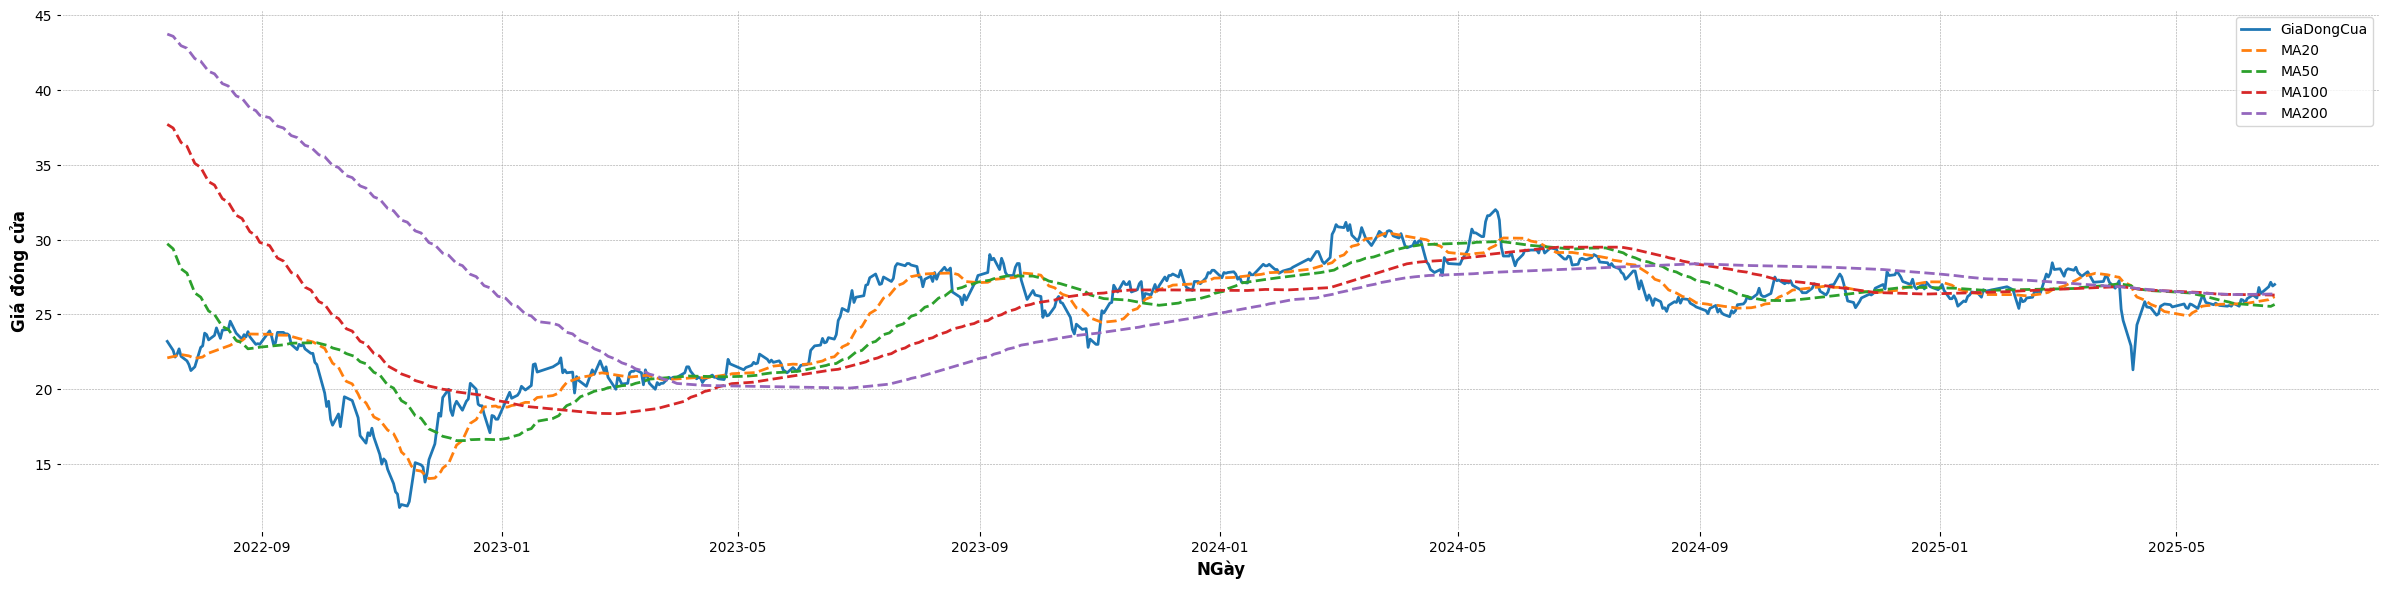
\includegraphics[width=0.90\textwidth]{images/TS_stock_close_MA.png}
        \caption{Giá đóng cửa 2 năm gần nhất cùng các đường MA}
        \label{fig:TS_stock_close_MA}
    \end{figure}
    \FloatBarrier

    Biểu đồ  \ref{fig:TS_stock_close_MA} thể hiện vai trò của các đường trung bình động (MA) trong việc phản ánh xu hướng giá theo thời gian. Đường MA20 đại diện cho xu hướng ngắn hạn, MA50 cho trung hạn và MA100, MA200 dài hạn. Giai đoạn đầu, cả MA20, MA50, MA100 và MA200 đều có xu hướng giảm mạnh, đặc biệt là MA100 và MA200 thể hiện rõ xu hướng giảm dài hạn của thị trường. Khi giá bắt đầu phục hồi từ đầu năm 2023, các đường MA ngắn hạn như MA20 và MA50 nhanh chóng điều chỉnh theo, lần lượt cắt lên các đường MA dài hạn, đây là dấu hiệu đảo chiều tích cực trong ngắn hạn. Trong khi đó, MA100 và MA200 mất độ dốc giảm và dần đi ngang, cho thấy đà giảm dài hạn đã chững lại. Từ giữa 2023 đến giữa 2025, các đường MA hội tụ gần nhau và đi ngang, phản ánh giai đoạn tích lũy và thiếu xu hướng rõ ràng. Điều này cho thấy thị trường bước vào trạng thái ổn định, không có lực tăng hay giảm mạnh rõ rệt trong trung và dài hạn.

    \begin{figure}[htp]
        \centering
        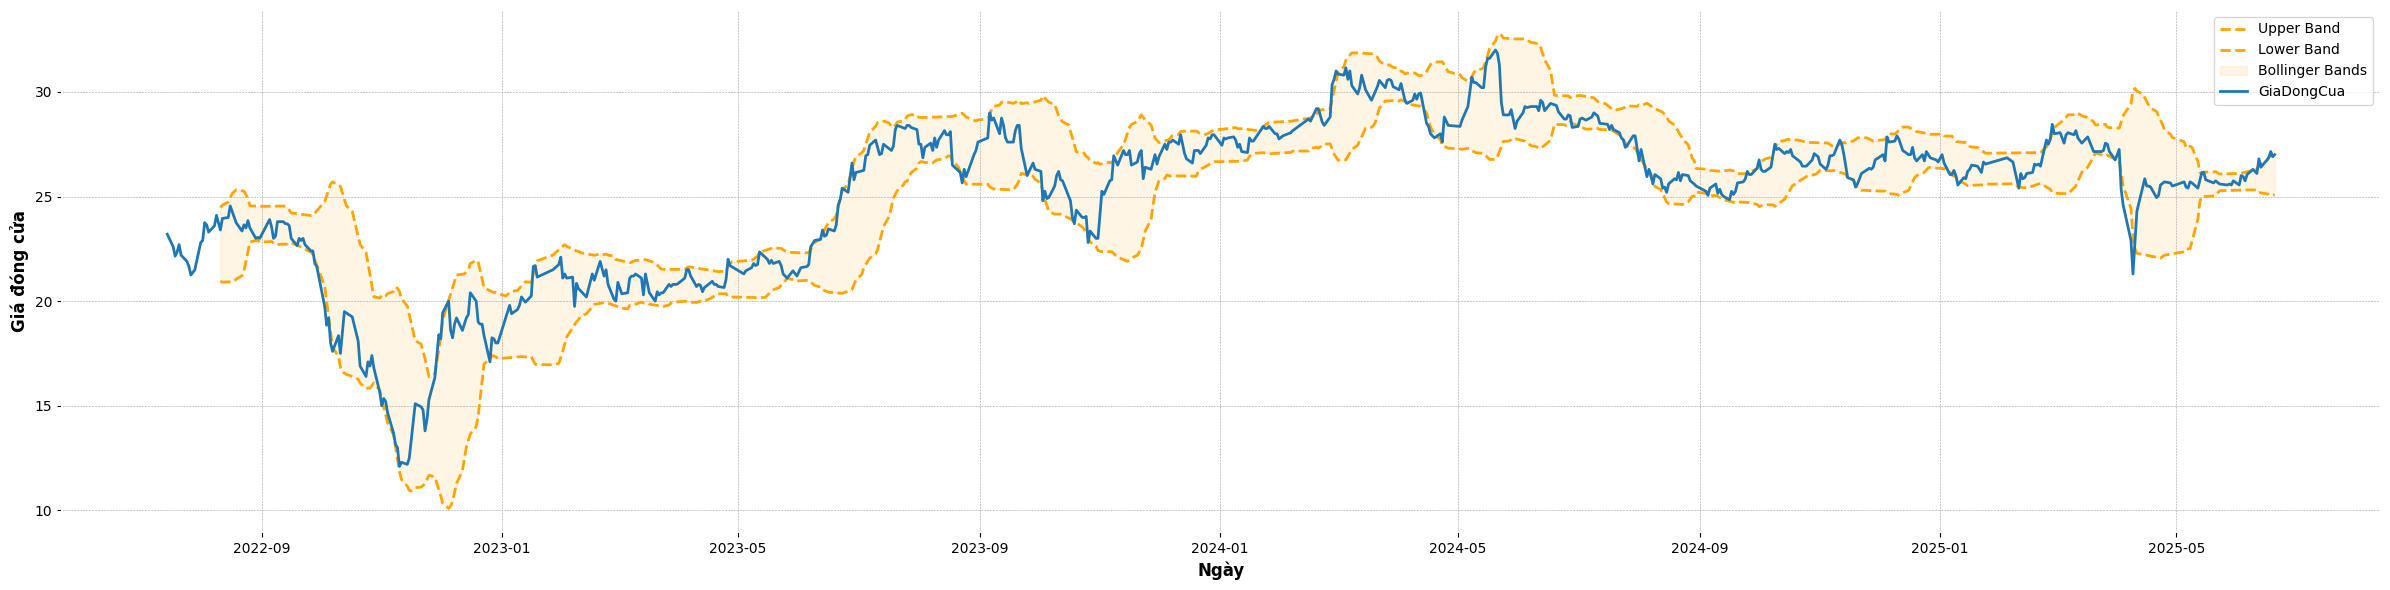
\includegraphics[width=0.90\textwidth]{images/TS_stock_bollinger.png}
        \caption{Giá đóng cửa 2 năm gần nhất cùng dải Bollinger bands}
        \label{fig:TS_stock_bollinger}
    \end{figure}
    \FloatBarrier

     Biểu đồ  \ref{fig:TS_stock_bollinger} cho thấy phần lớn thời gian giá dao động bên trong dải, tức là biến động vẫn nằm trong vùng bình thường. Có một số thời điểm vượt ra ngoài dải, như ở cuối năm 2022 và đầu năm 2025. Những lúc này, giá rơi mạnh xuống dưới dải dưới, phản ánh trạng thái quá bán trong ngắn hạn. Ngược lại, một vài giai đoạn như giữa năm 2023 và đầu 2024, giá vượt nhẹ lên trên dải trên, cho thấy thị trường tăng mạnh và có dấu hiệu quá mua. Ở các thời điểm đó, giá đều nhanh chóng quay lại vùng bên trong dải, cho thấy các pha vượt dải chỉ mang tính tạm thời và thường là dấu hiệu cho điều chỉnh hoặc đảo chiều ngắn hạn.

     \begin{figure}[htp]
        \centering
        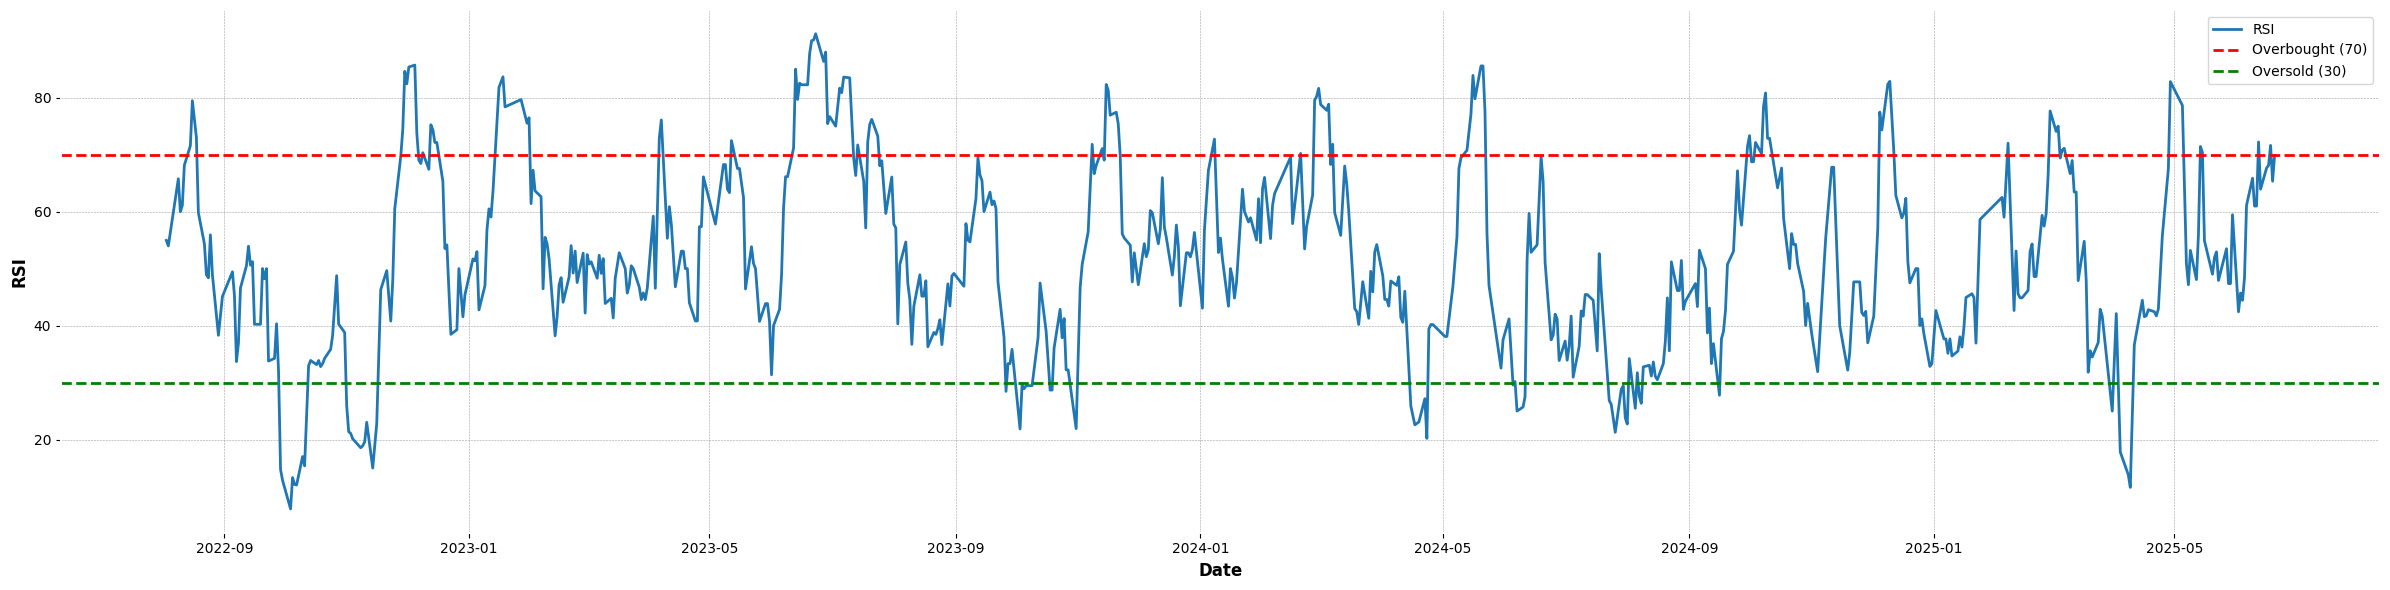
\includegraphics[width=0.90\textwidth]{images/TS_stock_RSI.png}
        \caption{RSI giá đóng cửa 2 năm gần nhất}
        \label{fig:TS_stock_RSI}
    \end{figure}
    \FloatBarrier

     Biểu đồ  \ref{fig:TS_stock_RSI} cho thấy đa số thời gian RSI dao động trong khoảng từ 30 đến 70, cho thấy thị trường chủ yếu ở trạng thái cân bằng, không quá nghiêng về một chiều tăng hay giảm. Những lần RSI vượt ngưỡng đều chỉ diễn ra ngắn hạn, sau đó nhanh chóng quay lại vùng trung lập. Điều này cho thấy xu hướng giá mang tính dao động ngắn hạn, chưa có dấu hiệu duy trì lực mua hoặc bán mạnh trong thời gian dài.

     \begin{figure}[htp]
        \centering
        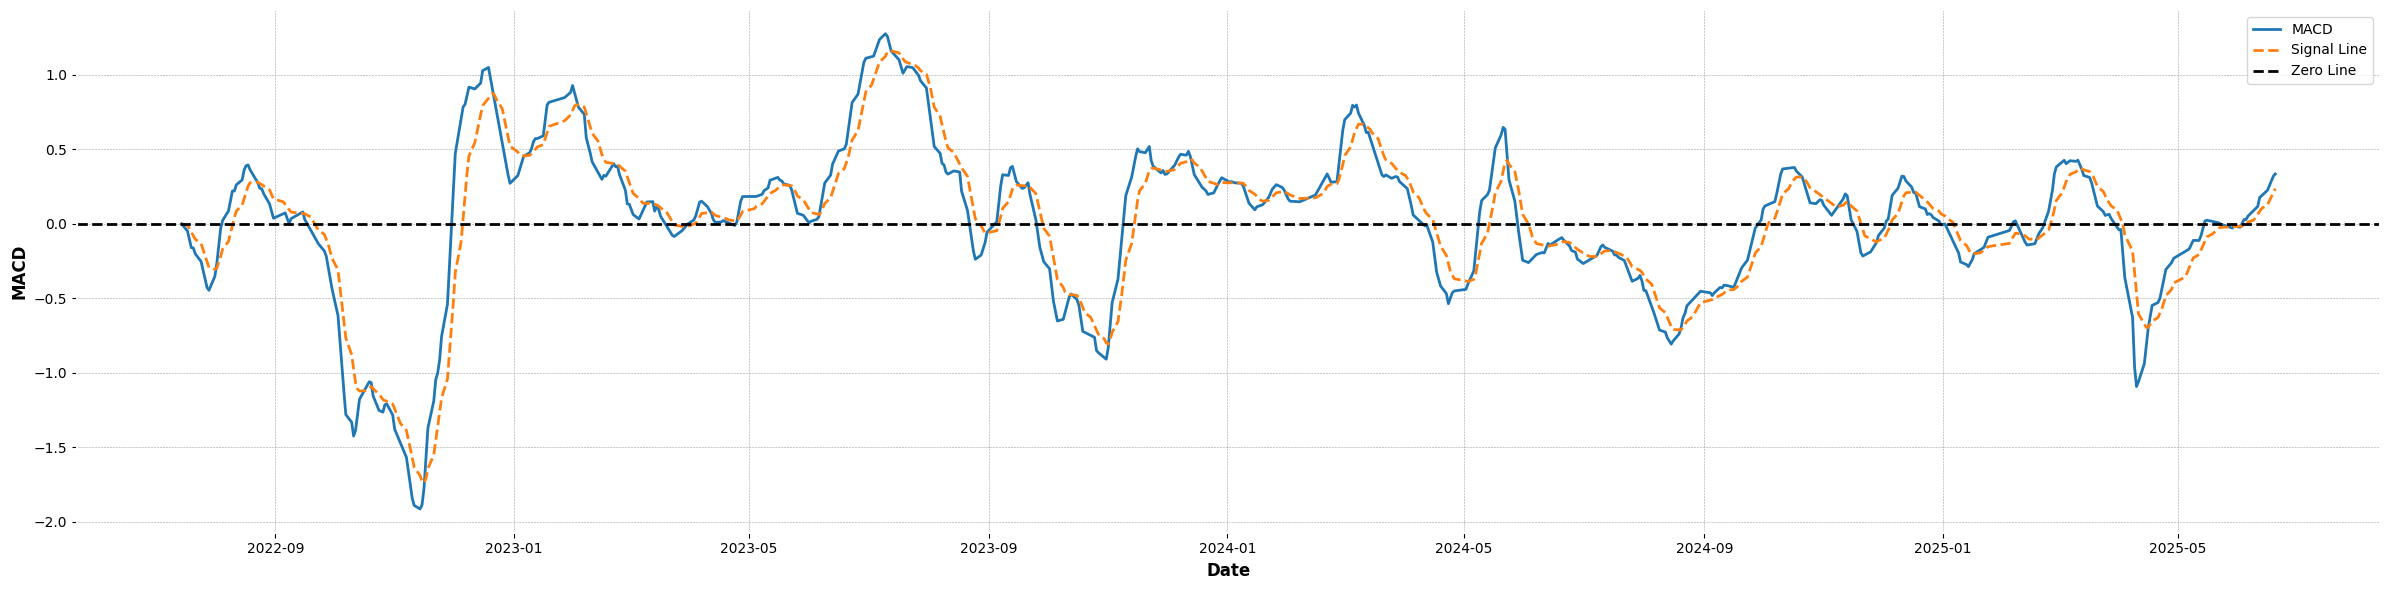
\includegraphics[width=0.90\textwidth]{images/TS_stock_MACD.png}
        \caption{MACD giá đóng cửa 2 năm gần nhất}
        \label{fig:TS_stock_MACD}
    \end{figure}
    \FloatBarrier

    Biểu đồ \ref{fig:TS_stock_MACD} thể hiện nhiều biến động của xu hướng giá đóng cửa. Giai đoạn cuối năm 2022 đến đầu 2023, MACD tăng mạnh và vượt ngưỡng 0, cho thấy tín hiệu tích cực từ thị trường. Tuy nhiên, sau đó đường này bắt đầu suy yếu và dao động quanh mức 0, phản ánh trạng thái thiếu xu hướng rõ ràng. Trong thời gian này, MACD liên tục cắt lên và cắt xuống đường tín hiệu (Signal Line), nhưng phần lớn các giao cắt đều diễn ra trong vùng trung tính, nên không tạo ra tín hiệu mua bán mạnh. Đặc biệt, trong nửa cuối giai đoạn, MACD chủ yếu nằm dưới Signal Line và dưới ngưỡng 0, cho thấy lực mua suy yếu và áp lực bán chiếm ưu thế hơn.

\subsubsection{Mô hình hóa dữ liệu}
    \paragraph{Cấu hình cài đặt} 
    \leavevmode

    Các mô hình sử dụng:

    \begin{itemize}
        \item \textbf{Linear Regression}: 

            \begin{lstlisting}[language=Python]
                LinearRegression()
            \end{lstlisting}

        \item \textbf{Random Forest Regressor}:

            \begin{lstlisting}[language=Python]
                RandomForestRegressor(
                    n_estimators=n_estimators, 
                    max_depth=max_depth, 
                    min_samples_leaf=min_samples_leaf
                )
            \end{lstlisting}

            khoảng hypertune tham số

            \begin{lstlisting}[language=Python]
                list_max_depth = [2, 3, 5, 10]
                list_n_estimators = [50, 100, 150, 200]
                list_min_samples_leaf = [1, 3, 5, 10]
            \end{lstlisting}.

        \item \textbf{XGBoost Classifier}:
            \begin{lstlisting}[language=Python]
                XGBRegressor(
                    n_estimators=n_estimators, 
                    max_depth=max_depth, 
                    reg_lambda=reg_lambda,
                    learning_rate=learning_rate,
                    reg_alpha=reg_alpha,
                )
            \end{lstlisting}

            khoảng hypertune tham số

            \begin{lstlisting}[language=Python]
                list_max_depth_xgb = [ 6, 7, 8]
                list_lambda = [0.5, 1, 2]
                list_learning_rate = [0.05, 0.1, 0.5]
                list_n_estimators_xgb  = [100, 150, 200]
                list_alpha = [0.5, 1]
            \end{lstlisting}.
        
    \end{itemize}

    Thuật toán data transform sử dụng: Standard Scaler.

    Chia tập dữ liệu huấn luyện: Train-Test: 80-20.

    \paragraph{Hồi quy giá đóng cửa 'GiaDongCua'}
    \leavevmode

    Chuyển đặc trưng 'GiaDongCua' và 'ThayDoiPhanTram' về dạng sliding window để dự đoán hồi quy, thử nghiệm trên các khoảng: 3, 7, 14, 21, 30, 90, 180, 365.

    Kết quả:
    \begin{itemize}
        \item \textbf{Linear Regression}: 
        
            Mô hình tốt nhất:
            \begin{itemize}
                \item Khoảng sliding window: 14
            \end{itemize}

            \begin{table}[htbp]
            \centering
            \caption{Kết quả Linear Regression}
            \label{tab:stock-close-lireg}
            \begin{tabular}{llrrr}
            \hline
             & Dataset & MAE & RMSE & MAPE \\
            \hline
            0 & Train & 0.715833 & 1.224575 & 1.779761 \\
            1 & Test & 0.413751 & 0.638391 & 1.579713 \\
            \hline
            \end{tabular}
            \end{table}
  
            
            \FloatBarrier

            \begin{figure}[htp]
                \centering
                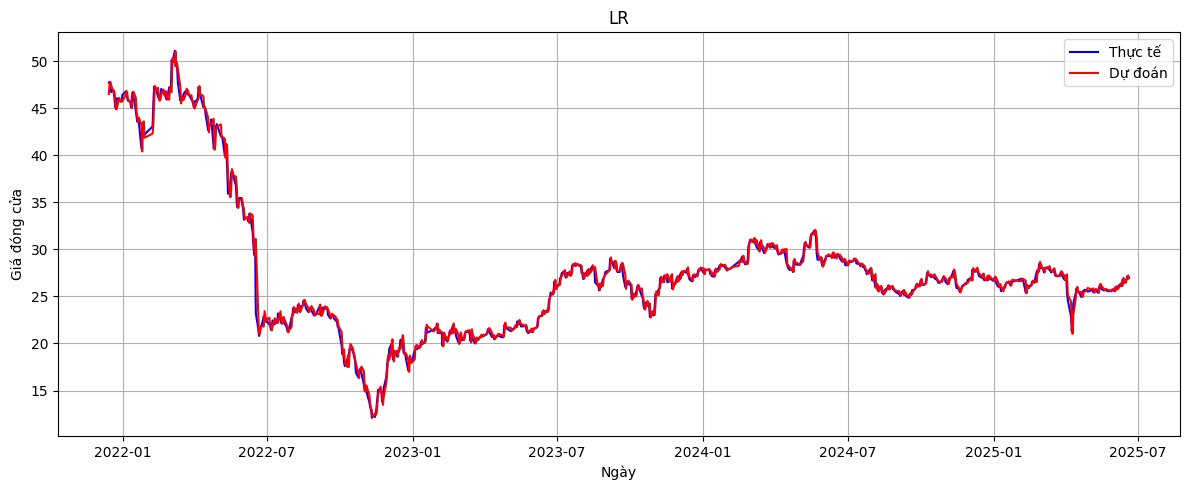
\includegraphics[width=0.90\textwidth]{images/TS_stock_pred_cmp_LR.png}
                \caption{Kết quả trên tập test Linear Regression}
                \label{fig:TS_stock_pred_cmp_LR}
            \end{figure}
        
            \FloatBarrier
            
        \item \textbf{Random Forest Regressor}:

            Mô hình tốt nhất:
            \begin{itemize}
                \item Khoảng sliding window: 3
                \item max\_depth: 10
                \item n\_estimators: 50
                \item min\_samples\_leaf: 3
            \end{itemize}

            \begin{table}[htbp]
                \centering
                \caption{Kết quả Random Forest Regressor}
                \label{tab:stock-close-rf}
                \begin{tabular}{llrrr}
                \hline
                 & Dataset & MAE & RMSE & MAPE \\
                \hline
                0 & Train & 0.525237 & 0.906095 & 1.304823 \\
                1 & Test & 0.473422 & 0.728184 & 1.908067 \\
                \hline
                \end{tabular}
            \end{table}
            
            \FloatBarrier

            \begin{figure}[htp]
                \centering
                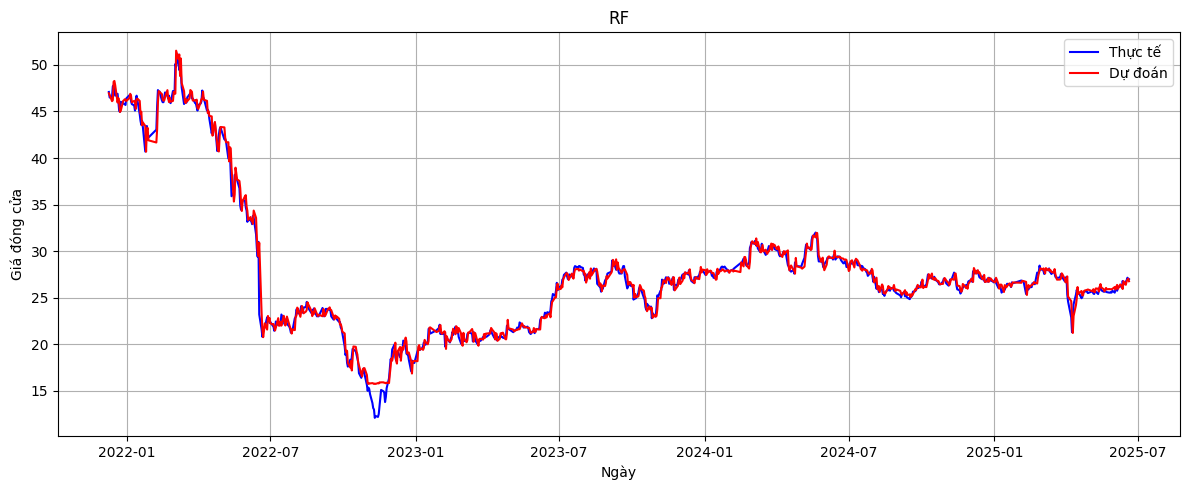
\includegraphics[width=0.90\textwidth]{images/TS_stock_pred_cmp_RF.png}
                \caption{Kết quả trên tập test RF Regressor}
                \label{fig:TS_stock_pred_cmp_RF}
            \end{figure}
            \FloatBarrier

        \item \textbf{XGBoost Regressor}:
        
            Mô hình tốt nhất:
            \begin{itemize}
                \item Khoảng sliding window: 3
                \item max\_depth: 6
                \item n\_estimators: 200
                \item reg\_lambda: 1
                \item reg\_alpha: 0.5
                \item learning\_rate: 0.05
            \end{itemize}

            \begin{table}[htbp]
                \centering
                \caption{Kết quả XGBoost Regressor}
                \label{tab:stock-close-xgb}
                \begin{tabular}{llrrr}
                \hline
                 & Dataset & MAE & RMSE & MAPE \\
                \hline
                0 & Train & 0.592337 & 0.918549 & 1.511546 \\
                1 & Test & 0.491972 & 0.833300 & 2.085304 \\
                \hline
                \end{tabular}
            \end{table}

            \FloatBarrier

            \begin{figure}[htp]
                \centering
                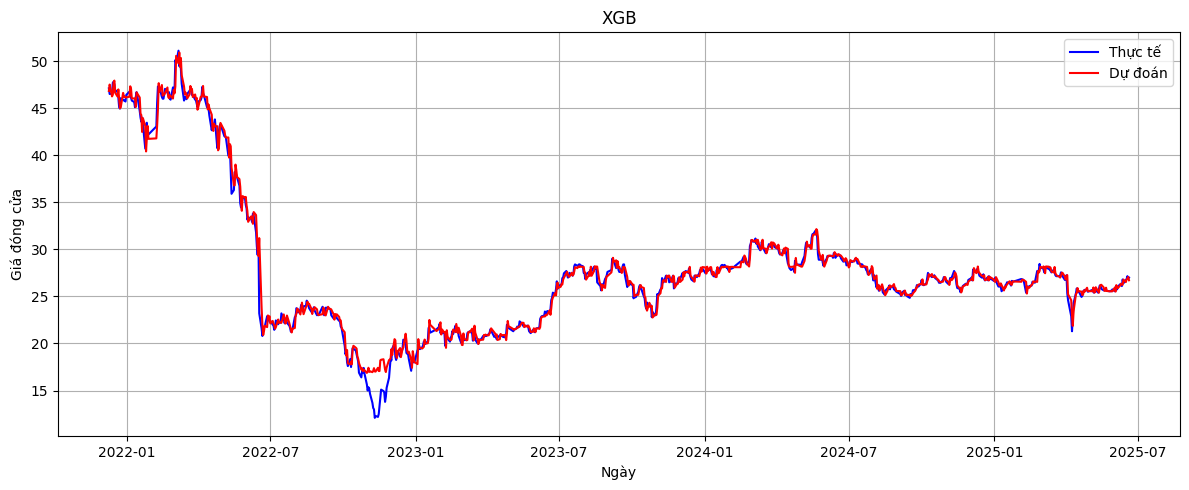
\includegraphics[width=0.90\textwidth]{images/TS_stock_pred_cmp_XGB.png}
                \caption{Kết quả trên tập test XGB Regressor}
                \label{fig:TS_stock_pred_cmp_XGB}
            \end{figure}
            \FloatBarrier
    \end{itemize}

    So sách các mô hình:

    \begin{table}[htbp]
        \centering
        \caption{So sánh kết quả các mô hình}
        \label{tab:stock-close-compare}
        \begin{tabular}{|l|c|c|c|}
        \hline
        Linear Regression & 0.419264 & 0.641979 & 1.610565 \\
        \hline
        Random Forest & 0.481274 & 0.745688 & 1.955963 \\
        \hline
        XGBoost & 0.544149 & 0.915723 & 2.370569 \\
        \hline
        \end{tabular}
    \end{table}

    \FloatBarrier

    Trong ba mô hình được đánh giá, Linear Regression cho thấy hiệu suất tốt nhất với các sai số thấp nhất trên tập kiểm tra (MAE = 0.419, RMSE = 0.642, MAPE = 1.61), cho thấy mô hình tuyến tính đơn giản này vẫn có thể nắm bắt tốt xu hướng trong dữ liệu chuỗi thời gian. Random Forest Regressor có độ chính xác thấp hơn so với Linear Regression, đặc biệt là ở chỉ số MAPE cao hơn đáng kể (1.96), mặc dù MAE và RMSE chỉ nhỉnh hơn một chút (lần lượt là 0.481 và 0.746). XGBoost Regressor là mô hình cho hiệu suất kém nhất trong ba phương pháp, với các sai số đều cao hơn, đặc biệt là MAPE (2.37), cho thấy chưa tận dụng được độ phức tạp của mô hình.

\subsubsection{Kết luận}
    Trong phần này, nhóm đã thực hiện phân tích và xây dựng các mô hình hồi quy nhằm dự đoán giá đóng cửa cổ phiếu HPG từ dữ liệu lịch sử. Sau khi xử lý dữ liệu và áp dụng kỹ thuật sliding window, ba mô hình Linear Regression, Random Forest Regressor và XGBoost Regressor đã được huấn luyện và so sánh. Kết quả cho thấy Linear Regression đạt hiệu suất tốt nhất trên tập kiểm tra, với sai số thấp hơn rõ rệt so với hai mô hình còn lại, phản ánh mối quan hệ tuyến tính giữa các phiên giao dịch có thể nắm bắt tốt xu hướng giá. Ngược lại, Random Forest và XGBoost tuy phức tạp hơn nhưng không mang lại độ chính xác cao hơn, đặc biệt MAPE lớn hơn đáng kể. Điều này cho thấy trong bối cảnh dự đoán ngắn hạn, mô hình đơn giản và cấu hình hợp lý vẫn có thể mang lại kết quả hiệu quả.